\documentclass{standalone}
\usepackage{diplomski}

\begin{document}

\chapter{Results} \label{ch:results}
\pagenumbering{arabic}
\setcounter{page}\thestranica

% --------------------------------------

The laboratory setup described in chapter \ref{ch:setup} enables simple change of measurement fibres, i.e. sensing elements, as well as use of different photodetectors. Here, different sets of single-mode and multi-mode fibres were tested. Different PIN photodiodes with electrical amplifiers and APD photodiodes, specified in Table \ref{table:photodetectors}, were tested. Additionally, different laser configurations and data processing algorithms were tested in the development process of the measurement system. This chapter reviews the obtained results, comparing the single-mode and multi-mode scenario.

\section{Single-mode fibres}

The first setup included single-mode fibres, connected in a manner displayed in Figure \ref{fig:smf_cascade}.
\begin{figure}[h]
	\centering
	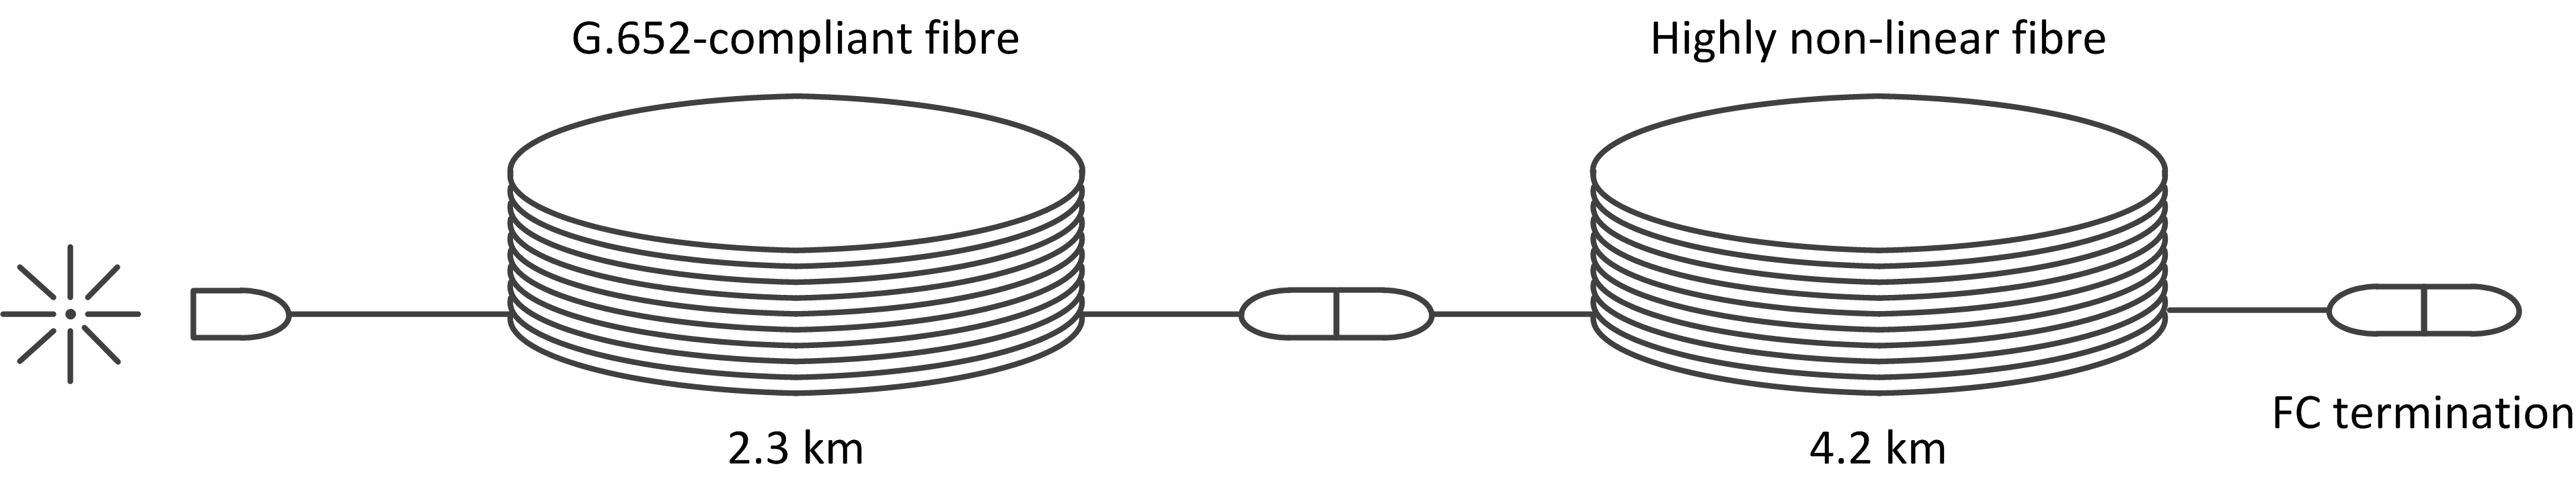
\includegraphics[width=\textwidth]{smf_cascade.png}
	\caption{Single-mode fibre cascade overview}
	\label{fig:smf_cascade}
\end{figure}
On the near side of the measurement and excitation equipment, a 2.3 km long roll of G.652-compliant single-mode fibre was connected. Its far end was spliced to a 4.2 km long roll of highly non-linear single-mode fibre. Such a fibre will yield a higher non-linear response to the incident optical signal \cite{Hiroishi2003}. In other words, lower power will be required to obtain the same SNR in the backscattered signal when using a highly non-linear fibre. A step in the scattered signal profile is visible, as a result of different $\left|\beta_3\right|$ and $\bar{n_2}$ coefficients, and of the reflection against SC-APC connectors between the fibres. Fibres were terminated with an FC terminator, designed to provide minimum reflection. \\

The first measurements were conducted with a simple data processing algorithm, which used only a classical averaging filter. SNR improvement with time is evident, although further measurements did not yield any better results. The averaging filter has probably reached its best result in terms of the final SNR, while it still remains a very slow solution for filtering the signals. The next step in developing the data processing algorithm was the implementation of an adaptive LMS filter. A comparison of results between the classical averaging filter and the adaptive LMS filter is given in Figure \ref{fig:classic_lms_compare}.
\begin{figure}[h]
	% Measurements 30.03.2017
	\begin{subfigure}[b]{0.49\textwidth}
		\begin{tabular}{c}
			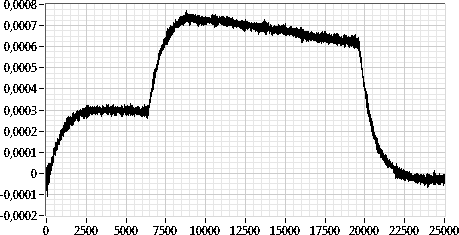
\includegraphics[width=\textwidth]{classic_lms_compare_stokes_classic.png} \vspace{1em} \\
			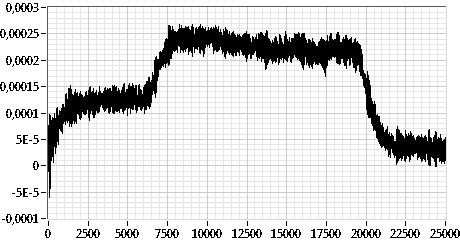
\includegraphics[width=\textwidth]{classic_lms_compare_antistokes_classic.png}
		\end{tabular}
		\caption{Classic averaging filter}
	\end{subfigure}
	\begin{subfigure}[b]{0.5\textwidth}
		\begin{tabular}{c}
			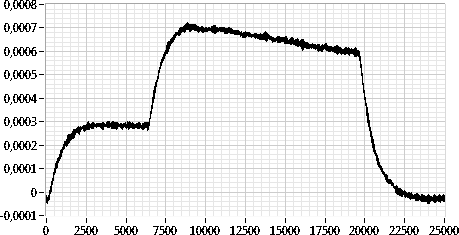
\includegraphics[width=\textwidth]{classic_lms_compare_stokes_lms.png} \vspace{1em} \\
			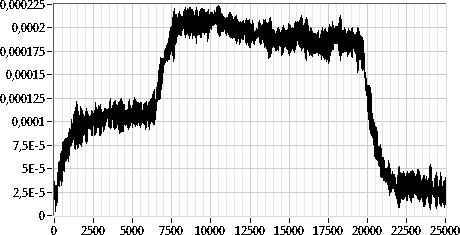
\includegraphics[width=\textwidth]{classic_lms_compare_antistokes_lms.png}
		\end{tabular}
		\caption{Adaptive LMS filter}
	\end{subfigure}
	\caption{A comparison of filters with Stokes signal (top) and anti-Stokes signal (bottom)}
	\label{fig:classic_lms_compare}
\end{figure}
The presented results are obtained with an averaging time of 7 minutes. While the results are very similar, certain features of the adaptive LMS algorithm need to be considered. Firstly, in the anti-Stokes graph, the adaptive LMS filter has managed to extract finer features of the scattered profile. While the SNR for the anti-Stokes profile remains roughly the same, higher spectral components that may be the result of an actual feature of the physical quantity of interest, have passed through the adaptive LMS filter. Also, it is important to note that the same SNR was achieved with the adaptive LMS filter much sooner than with the classic averaging filter. The graph presented in \ref{fig:classic_lms_compare}, displaying data from the adaptive LMS filter, had converged to its final form in less than one minute, dramatically decreasing the required measurement time. \\

Whilst observing the scattering profiles, one must estimate the maximum incident optical power that is still below the stimulated Raman scattering threshold. In all measurements, the first laser EDFA had a constant pump power
\begin{equation} \label{eq:edfa_first_pump}
I_1 = \SI{400}{\milli \ampere} \textrm{.}
\end{equation}
The lower setting of the first pump power ensured small ASE, although this has been further filtered, as described in chapter \ref{ch:setup}. The second pump power was swept, and the peak optical power measured. The qualitative rating of the waveform, as well as the estimated temperature inaccuracy is presented in Table \ref{table:smf_power_sweep}.
\begin{table}[t]
	\centering
	\caption{Sweeping optical power with an SM fibre}
	\label{table:smf_power_sweep}
	\begin{tabular}{C{2.5cm}|C{2.5cm}|C{2cm}|C{5cm}}
		\textbf{Pump current [mA]} & \textbf{Pulse peak power [mW]} & \textbf{$\bm{\varDelta T}$ [K]} & \textbf{Qualitative rating} \\
		\hline \hline
		600 & 730 & 200 & Profile visible \\
		700 & 2300 & 75 & -- \\
		800 & 3000 & 30 & -- \\
		900 & 3920 & 20 & Visible peak at the end of the profile \\
		1000 & 5540 & 15 & -- \\
		1050 & 6565 & 10 & Highly expressed peak at the end of the profile
	\end{tabular}
\end{table}
Pulse duration was set to 50 ns, and the measurement time was under 1 minute. A number of observations can be made here. Firstly, it can be seen that the pump power and the optical power have an irregular relation for this laser. In fact, the laser lacks power regulations, so the once set optical power was often unrepeatable, in spite the same configuration. After some finer measurements, it was observed that a setting of
\begin{equation}
I_{2,\textrm{max}} = \SI{1010}{\milli \ampere}
\end{equation}
yielding an optical power of about
\begin{equation}
P_\textrm{max} = \SI{5800}{\milli \watt}
\end{equation}
was a repeatable maximum power setting before the effects of SRS become significant. \\

Next, the laser impulse width was swept in order to determine the effect this will have to the measurement inaccuracy. It was shown that the width itself has little effect on the inaccuracy of the measured value itself. It is, however, important to ensure that the laser width is long enough so the photodetectors, with their limited bandwidth, faithfully represent the impulse waveform and amplitude. Laser's pulse width can be configured in steps of 2.5 ns, and a value of
\begin{equation}
T_{0,\textrm{min}} = \SI{12.5}{\nano \second}
\end{equation}
was determined as the minimal required pulse width. In principle, shorter pulse width provides a finer spatial resolution, according to \ref{eq:otdr_resolution}. However, due to filtering nature of the decimation procedure performed on the calculated temperature profile, selecting a lower resolution will in fact yield a \textit{smoother} temperature profile. This is further discussed in the multi-mode scenario, where more comparative measurements were made. For many future measurements, a pulse width of
\begin{equation}
T_0 = \SI{25}{\nano \second}
\end{equation}
was selected as a representative configuration, yielding a spatial resolution of
\begin{equation}
z_0 = \SI{2.5}{\meter} \textrm{.}
\end{equation} \\

The final configuration parameter is the laser pulse repetition rate. Intuitively, we wish to have a rate that is large enough to provide a sufficient number of measurements in a given time frame, so that data averaging can be effective. For most measurements, the repetition rate was set to
\begin{equation}
f_R = \SI{1}{\kilo \hertz} \textrm{.}
\end{equation}
Data processing software is not that fast. The runtime of a single processing iteration is estimated to be around 10--15 ms. Normally, setting a larger repetition rate would not pose a problem, as the software would only process the data that is last acquired from the DAQ card. However, architecture of the DAQ system needs to be taken into account. As the National Instruments PXIe-5160 has its own acquisition buffer memory, it is capable of performing the data acquisition when triggered, even if a large amount of data is still buffered and not transferred to the LabVIEW environment \cite{datasheet:daq}. A considerable back-log could occur, and software would continue running the data acquisition loop long after the laser output was turned off. On the other hand, some hanging of data acquisition software was noticed when setting the repetition rate too high. This could be a result of DAQ card's FIFO memory being overflown while the first data was still being transferred to the LabVIEW software. While fine-tuning the DAQ part of the software, a repetition rate of
\begin{equation}
f_R = \SI{100}{\hertz}
\end{equation}
was found to be sufficient for this purpose. \\

An example of the final measurement, at maximum allowable optical power, is given in Figure \ref{fig:smf_final}.
\begin{figure}[h]
	% Measurement 13.04.2017
	\centering
	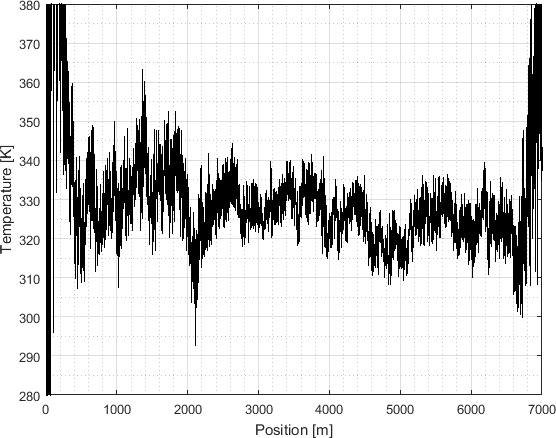
\includegraphics[width=0.8\textwidth]{smf_final.png}
	\caption{SMF temperature measurement}
	\label{fig:smf_final}
\end{figure}
It is clear that only the highly non-linear fibre yields results with a reasonable accuracy, measured by this example to be about 
\begin{equation}
\varDelta T_\textrm{SMF} \approx \SI{20}{\kelvin} \textrm{.}
\end{equation}
Further data processing is expected to be able to bring the accuracy down to about 10 K. Measurements were made by PDA10CS-EC photodetectors, with the gain setting set to 40 dB. Therefore, we may expect some rapid temperature changes not to be detected by the system, as this setting provides a very narrow bandwidth. However, the problem with this setup is the accuracy of the sensing element itself, and future use of single-mode fibres was abolished. It should be noted that calibration against the discrete temperature sensor was not implemented in LabVIEW at this point, so the measured temperature profile has an offset against the actual fibre temperature.

\section{Multi-mode fibres}

As the effective cross-section area of a multi-mode fibre is larger than that of a single-mode fibre, the former is expected to demonstrate better sensing performance and temperature accuracy for this system. Larger cross-section area of fibre core produces lower power densities at a constant power level. According to \ref{eq:raman_threshold}, multi-mode fibres will, therefore, be able to withstand higher peak optical powers before reaching SRS threshold. \\

As described in chapter \ref{ch:setup}, a lot of the optical components were changed in the multi-mode scenario, to ensure best coupling of incident optical power, and capturing of backscattered power. For the first multi-mode setup, a cascade of two G.651-compliant fibres was used. The setup is presented in Figure \ref{fig:mmf_first_cascade}.
\begin{figure}[h]
	\centering
	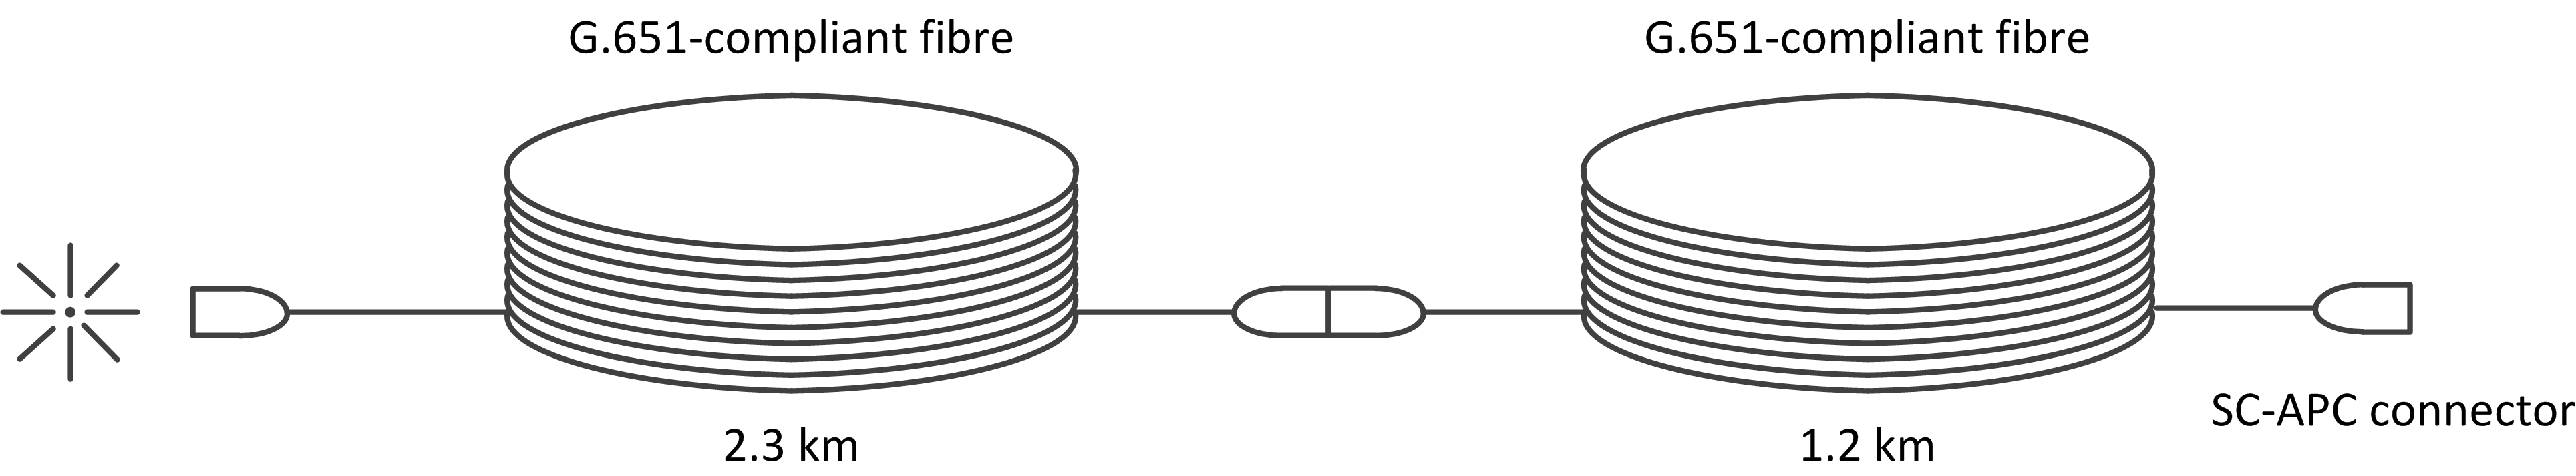
\includegraphics[width=\textwidth]{mmf_first_cascade.png}
	\caption{Initial multi-mode fibre cascade overview}
	\label{fig:mmf_first_cascade}
\end{figure}
The first fibre was 2.3 km, and the second 1.2 km in length. The two fibres were initially connected by SC-APC connectors, and terminated by another SC-APC connector with no matched termination at the end. \\

Different photodetectors were used in this setup. First measurements were performed with PDA10CS-EC with switchable gain. Firstly, the 40 dB setting was used to find the maximum peak optical power this system could use. Laser's first EDFA pump current was set as in \ref{eq:edfa_first_pump}, while the second EDFA pump current was swept. The qualitative rating of the waveform, and the estimated temperature inaccuracy is presented in Table \ref{table:mmf_power_sweep}.
\begin{table}[h]
	\centering
	\caption{Sweeping optical power with an MM fibre}
	\label{table:mmf_power_sweep}
	\begin{tabular}{C{2.5cm}|C{2.5cm}|C{2cm}|C{5cm}}
		\textbf{Pump current [mA]} & \textbf{Pulse peak power [mW]} & \textbf{$\bm{\varDelta T}$ [K]} & \textbf{Qualitative rating} \\
		\hline \hline
		1000 & 5600 & >10 & Profile clearly visible \\
		1100 & 9600 & <10 & -- \\
		1200 & 13500 & 5--10 & -- \\
		1250 & 15400 & <5--8 & High reflection off the end of the fibres
	\end{tabular}
\end{table}
Multi-mode fibres have proven to be capable of using higher optical powers without inducing SRS, as was expected. Once again, a step in scattering profiles is visible, as a result of reflection against SC-APC connectors between the fibres. This problem will be solved by splicing the two fibres later on. A sample scattering profile is shown in Figure \ref{fig:mmf_scatters}. Comparative temperature measurements at two optical powers are also given, in Figure \ref{fig:mmf_power_temperatures}.
\begin{figure}[b!]
	% Measurement 19.04.
	\centering
	\begin{subfigure}[b]{0.49\textwidth}
		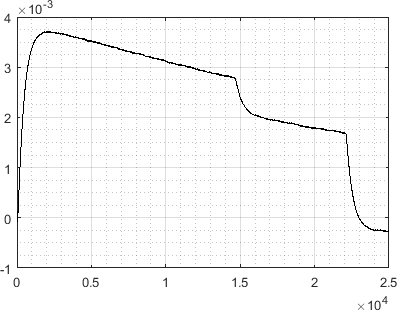
\includegraphics[width=\textwidth]{mmf_scatters_stokes.png}
		\caption{Stokes component}
	\end{subfigure}
	\begin{subfigure}[b]{0.49\textwidth}
		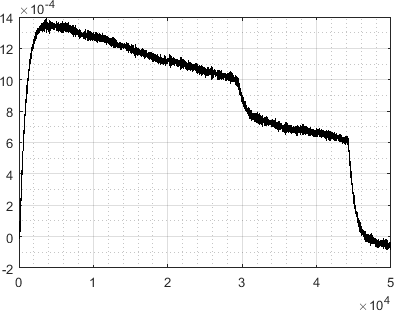
\includegraphics[width=\textwidth]{mmf_scatters_antistokes.png}
		\caption{Anti-Stokes component}
	\end{subfigure}
	\caption{Scattering profiles at incident optical power $P = \SI{9.7}{\watt}$}
	\label{fig:mmf_scatters}
\end{figure}
\begin{figure}[h]
	% Measurement 19.04.
	\centering
	\begin{subfigure}[b]{0.49\textwidth}
		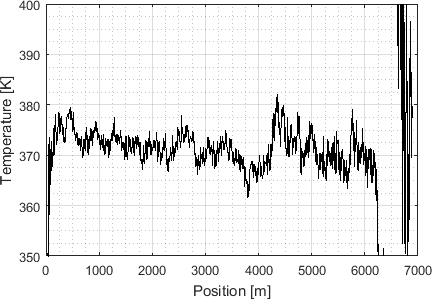
\includegraphics[width=\textwidth]{mmf_power_temperatures-01.png}
		\caption{$P = \SI{5.47}{\watt}$}
	\end{subfigure}
	\begin{subfigure}[b]{0.49\textwidth}
		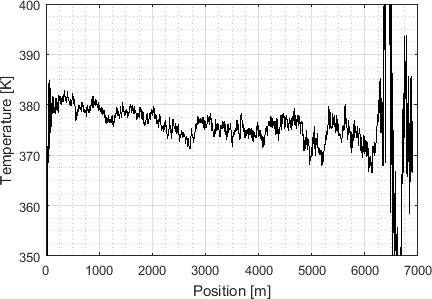
\includegraphics[width=\textwidth]{mmf_power_temperatures-2-02.png}
		\caption{$P = \SI{9.65}{\watt}$}
	\end{subfigure}
	\caption{Measured uncalibrated temperatures at different optical powers}
	\label{fig:mmf_power_temperatures}
\end{figure}
It is clear that multi-mode fibres provide much better measurement performance, compared to single-mode fibres. Note that the same or better performance is obtained with standard a multi-mode fibre, in comparison to a highly non-linear single-mode fibre. The achieved temperature accuracy is estimated to be 
\begin{equation}
\varDelta T < \SI{5}{\kelvin} \textrm{.}
\end{equation}
Some problems still occur at the end of the measurement region, but these are predominantly the result of poor fibre termination. \\

Further measurements were made to evaluate the quality of photo-detection diodes. Firstly, PIN diodes PDA10CS-EC were tested, especially with the far weaker anti-Stokes scattering signal. Different gains, and thus different bandwidths, were used to determine the best possible configuration. On the anti-Stokes channel, only the 30 dB and 40 dB options were concluded to provide reasonable measurements. However, waveform deterioration on higher-gain setting was evident. On Stokes channel, even the 20 dB gain setting was sufficient to maintain a reasonable SNR, whilst reproducing waveform features well. The only viable solution for anti-Stokes channel was the use of an APD diode, but the implementation was delayed. Some other interim measurements were performed, with a 40 dB setting on PIN diode amplifiers. \\

The next step was adding a patch cable between the two cascaded fibres, as shown in Figure \ref{fig:mmf_second_cascade}.
\begin{figure}[h]
	\centering
	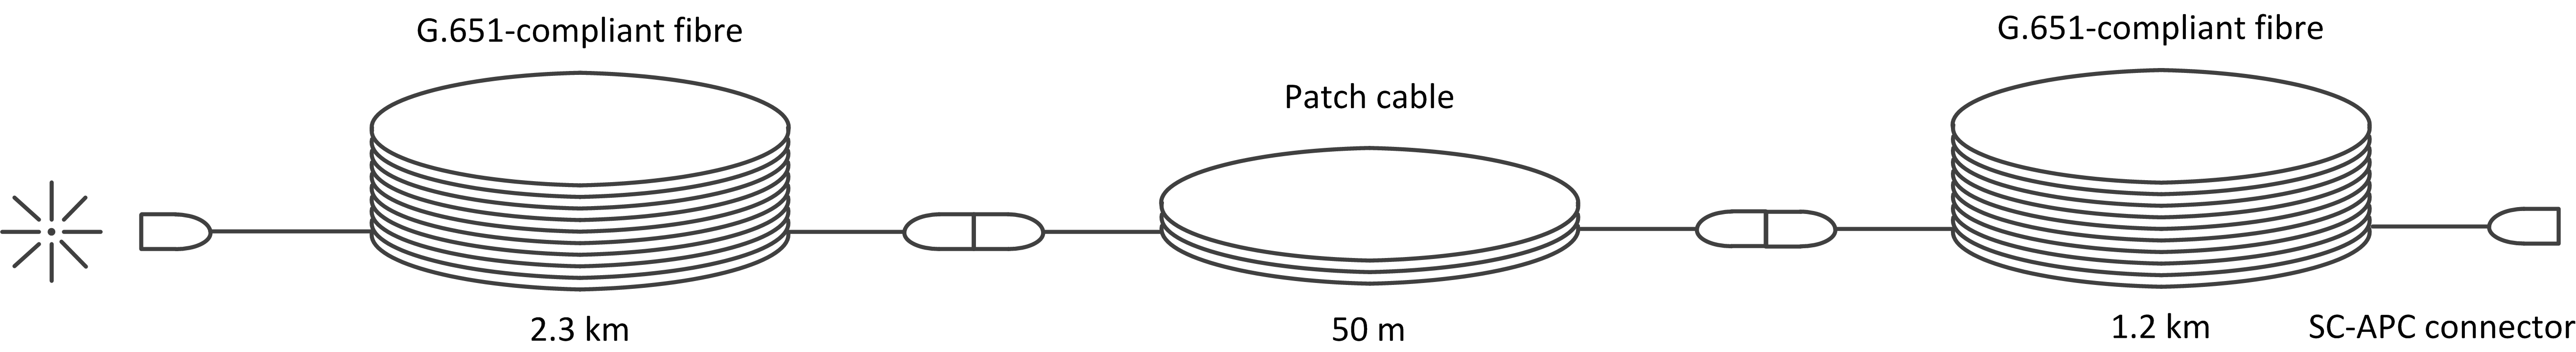
\includegraphics[width=1\textwidth]{mmf_second_cascade.png}
	\caption{Second multi-mode fibre cascade overview}
	\label{fig:mmf_second_cascade}
\end{figure}
The patch is 50 m in length. It was inserted to serve as a stretch that will be subjected to heating and cooling, in order to measure system performance with different temperatures along the line. Therefore, the patch was kept in full standard shielding to enable safe temperature control. The middle position in the system was chosen to ensure no unwanted effects from reflections against fibre ends would occur, obscuring the actual measurement result. All three system parts were spliced together, eliminating reflections. The immediate effect is visible in scattering profiles. The step-like behaviour has disappeared, proving that the splices have minimum losses. \\

The patch cable was now heated to about \SI{50}{\celsius}. The scattered signals and temperature profile are displayed in Figure \ref{fig:first_50c}.
\begin{figure}[h!]
	\begin{subfigure}[b]{0.49\textwidth}
		\flushleft
		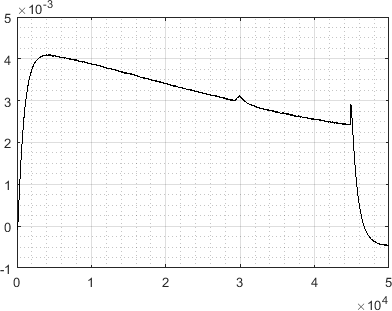
\includegraphics[width=\textwidth]{first_50c_stokes.png}
		\caption{Stokes component}
		\vspace{1em}
	\end{subfigure}
	\begin{subfigure}[b]{0.49\textwidth}
		\flushright
		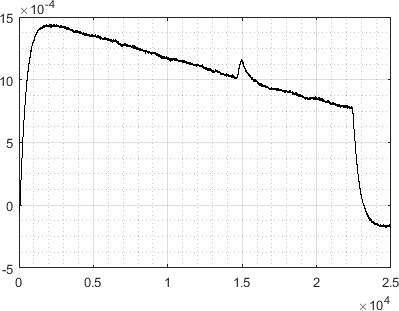
\includegraphics[width=\textwidth]{first_50c_antistokes.png}
		\caption{Anti-Stokes component}
		\vspace{1em}
	\end{subfigure}
	\begin{subfigure}[b]{\textwidth}
		\centering
		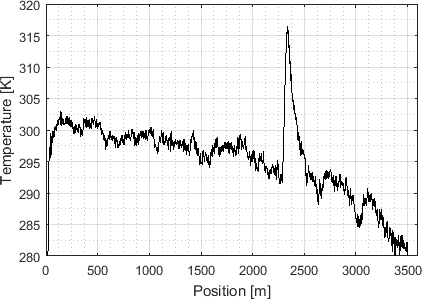
\includegraphics[width=0.8\textwidth]{first_50c_temp.png}
		\caption{Temperature profile}
	\end{subfigure}
	\caption{Measuring fibre patch heated to \SI{50}{\celsius}}
	\label{fig:first_50c}
\end{figure}
The temperature profile clearly and accurately shows the temperature difference between fibre parts. Some problems are also evident. The first is the width of the temperature step. Although the patch length is 50 m, and only the patch was heated, the measured temperature shift has an apparent relaxation that \textit{runs} for about 200 effective metres. As the amplifiers for PIN diodes were set to the 40 dB gain option, their bandwidth was mere \SI{320}{\kilo \hertz}, which was considered insufficient to properly measure rapid temperature changes. A reading from the discrete temperature sensor was now implemented as a calibration mechanism. Therefore, the temperature at the beginning of the calculated profile corresponds to the actual room temperature, which most of the measurement fibres were in. However, due to errors in temperature calculation term, caused by the reasons already discussed in chapter \ref{ch:data_processing}, the temperature profile exhibits a constant slope. So, the absolute temperature error at the end of the measurement fibre is 
\begin{equation}
\varDelta T_\textrm{total} \approx \SI{15}{\kelvin} \textrm{.}
\end{equation}
PIN diodes were thus identified as the limiting component of the current measurement system. Therefore, a more sensitive component had to be implemented, especially on the anti-Stokes channel. \\

The next step was, therefore, implementing an APD-based photodetector on the anti-Stokes channel. The model used was APD130C by Thorlabs. Its characteristics and calibration procedure were presented in chapter \ref{ch:setup}. The diode is declared to have very low noise, high responsivity and large bandwidth, making it ideal for monitoring weak anti-Stokes scattered signals. After calibrating the APD diode, the PIN-based photodetector monitoring Stokes scattering was re-configured to the 20 dB gain option, in order to increase bandwidth. A new measurement was made at room temperature. Additionally, a core-less termination fibre was spliced to the end of the measurement cascade. The termination fibre reduced reflection off the system end, and the spikes previously found at the end of scattering profiles were almost completely reduced. The measurement is displayed in Figure \ref{fig:apd_scattering}.
\begin{figure}[h]
	% Measurement 12.06.
	\begin{subfigure}[b]{0.49\textwidth}
		\flushleft
		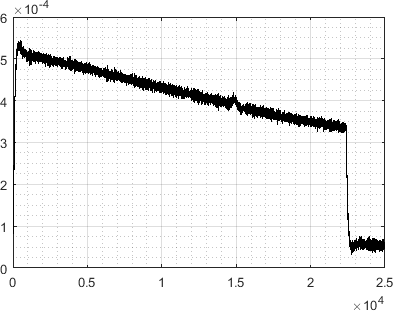
\includegraphics[width=0.99\textwidth]{apd_scattering_stokes}
		\caption{Stokes component}
	\end{subfigure}
	\begin{subfigure}[b]{0.49\textwidth}
		\flushright
		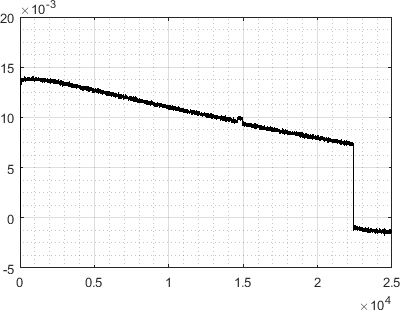
\includegraphics[width=0.99\textwidth]{apd_scattering_antistokes.png}
		\caption{Anti-Stokes component}
	\end{subfigure}
	\caption{Measurement with an APD diode at the anti-Stokes channel}
	\label{fig:apd_scattering}
\end{figure}
At this point, the anti-Stokes measurement exhibits even better SNR than the Stokes measurement. This is due to a relatively low gain on the PIN diode-side. Nevertheless, this gain-configuration option was left intact, so as not to deteriorate the large bandwidth enabled by the APD diode. The low-bandwidth limitation of the PIN diode was still visible after heating the fibre patch to about \SI{60}{\celsius} and inspecting the measurement result shown in Figure \ref{fig:apd_60c}.
\begin{figure}[h!]
	% Measurement 12.06.
	\begin{subfigure}[b]{0.49\textwidth}
		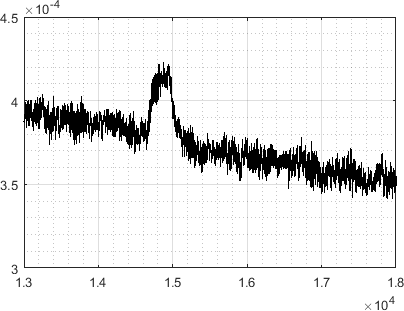
\includegraphics[width=\textwidth]{apd_60c_stokes.png}
		\caption{Stokes component}
		\vspace{1em}
	\end{subfigure}
	\begin{subfigure}[b]{0.49\textwidth}
		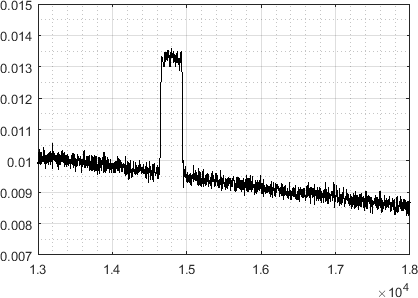
\includegraphics[width=\textwidth]{apd_60c_antistokes.png}
		\caption{Anti-Stokes component}
		\vspace{1em}
	\end{subfigure}
	\begin{subfigure}[b]{\textwidth}
		\centering
		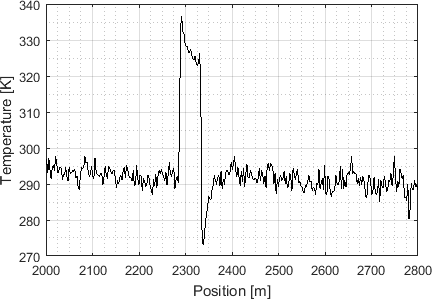
\includegraphics[width=0.8\textwidth]{apd_60c_temp.png}
		\caption{Temperature profile}
		\label{fig:apd_60c_temp}
	\end{subfigure}
	\caption{Measuring fibre patch heated to \SI{60}{\celsius}}
	\label{fig:apd_60c}
\end{figure}
The Stokes profile still features a relaxation after the step, and the resulting temperature profile has a subsequent error at the beginning and at the end of the patch. It is, therefore, concluded that a high-bandwidth APD diode is an advisable option for the Stokes channel, as well. Nevertheless, the achieved measurement performance was satisfactory. Final temperature inaccuracy of the implemented system was
\begin{equation}
\varDelta T \approx \SI{5}{\kelvin} \textrm{,}
\end{equation}
which proved the validity of using a multi-mode fibre for this application. \\

For the final approval of the selected configuration, a measurement sweep at different temperature was made by using different laser pulse widths. The result in Figure \ref{fig:apd_60c_temp} was obtained with a pulse width of $T_0 = \SI{25}{\nano \second}$. Figure \ref{fig:width_sweep_60c} represents measured temperature of \SI{60}{\celsius} for two other pulse widths.
\begin{figure}[h]
	% Measurement 13.06.
	\centering
	\begin{subfigure}[b]{0.49\textwidth}
		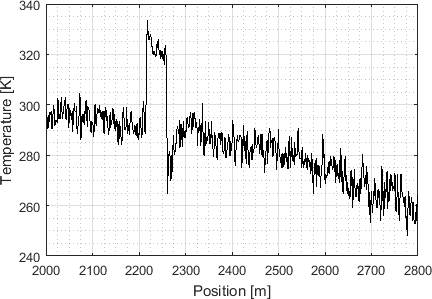
\includegraphics[width=\textwidth]{width_sweep_60c_12ns.png}
		\caption{$T_0 = \SI{12.5}{\nano \second}$}
	\end{subfigure}
	\begin{subfigure}[b]{0.49\textwidth}
		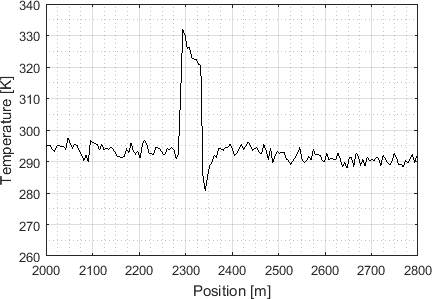
\includegraphics[width=\textwidth]{width_sweep_60c_50ns.png}
		\caption{$T_0 = \SI{50}{\nano \second}$}
	\end{subfigure}
	\caption{Measuring fibre patch heated to \SI{60}{\celsius} with different laser pulse widths}
	\label{fig:width_sweep_60c}
\end{figure}
Short pulses clearly degrade performance, due to photodetector bandwidth limitation. Longer pulses change the spatial resolution, but the overall performance remains the same. \\

The final set of graphs in Figure \ref{fig:final_measurements} presents measurements for different high and low temperatures.
\begin{landscape}
	\begin{figure}[h]
		% Measurement 13.06. and 14.06.
		\centering
		\begin{subfigure}[b]{0.49\linewidth}
			\centering
			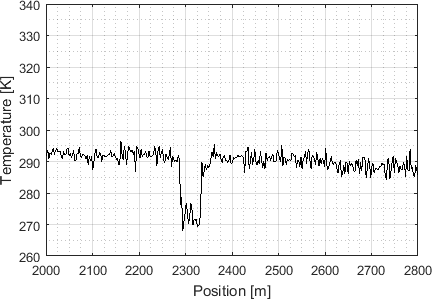
\includegraphics[width=0.8\textwidth]{final_measurements_-2c.png}
			\caption{$T = \SI{-2}{\celsius}$}
			\vspace{1em}
		\end{subfigure}
		\begin{subfigure}[b]{0.49\linewidth}
			\centering
			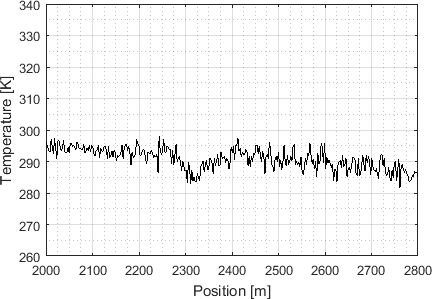
\includegraphics[width=0.8\textwidth]{final_measurements_10c.png}
			\caption{$T = \SI{10}{\celsius}$}
			\vspace{1em}
		\end{subfigure}
		\begin{subfigure}[b]{0.49\linewidth}
			\centering
			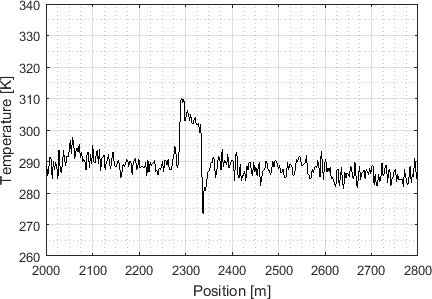
\includegraphics[width=0.8\textwidth]{final_measurements_40c.png}
			\caption{$T = \SI{40}{\celsius}$}
		\end{subfigure}
		\begin{subfigure}[b]{0.49\linewidth}
			\centering
			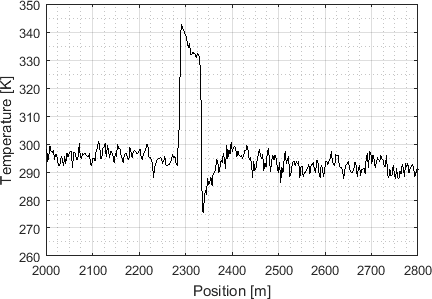
\includegraphics[width=0.8\textwidth]{final_measurements_70c.png}
			\caption{$T = \SI{70}{\celsius}$}
		\end{subfigure}
		\caption{Temperature measurements of the patch fibre}
		\label{fig:final_measurements}
	\end{figure}
\end{landscape}

\setcounter{page}{\thepage-1}

% --------------------------------------

\setcounter{stranica}{\thepage}
\addtocounter{stranica}{1}

\end{document}